\documentclass[9pt,onecolumn,twoside]{pnas-new}
% Remove the twocolumn option to create a single column SI file if required.
% Use the lineno option to display guide line numbers if required.
% Note that the use of elements such as single-column equations
% may affect the guide line number alignment.

\templatetype{pnassupportinginfo}
\usepackage{listings}
\lstset{basicstyle=\ttfamily,
  showstringspaces=false,
  commentstyle=\color{red},
  keywordstyle=\color{blue}
}
\title{Supporting Information}
\author{Hough et al.}

\doi{genetics.XXXXXXXXXX}

\begin{document}

\maketitle

%\section*{Supporting Information (SI)}

\section*{SI Tables}

\begin{table}[tbhp!]
\centering
\caption{Population identities (ID) and location information for \textit{R. hastatulus} samples}
\begin{tabular}{lllll}
Population ID & Location & Altitude & Latitude & Longitude \\
\midrule
\textbf{Texas} &  &  &  &  \\
TX-MTP & Mount Pleasant, Texas & 130	 & 33.17453 & 94.98799 \\
OK-RAT & Rattan, Oklahoma & 138 & 34.15755 & 95.41325 \\
TX-LIV & Livingston, Texas & 83 & 30.69947 & 94.79981 \\
LA-DER & De Ridder, Lousiana & 67 & 30.8941 & 93.3143 \\
TX-ATH & Athens, Texas & 145 & 32.18471 & 95.8032 \\
OK-WIL & Willis, Oklahoma & 211 & 33.89663 & 96.83533 \\
\bottomrule
\end{tabular}
\end{table}

\section*{SI Figures}

\begin{figure}[tbhp!]
\centering
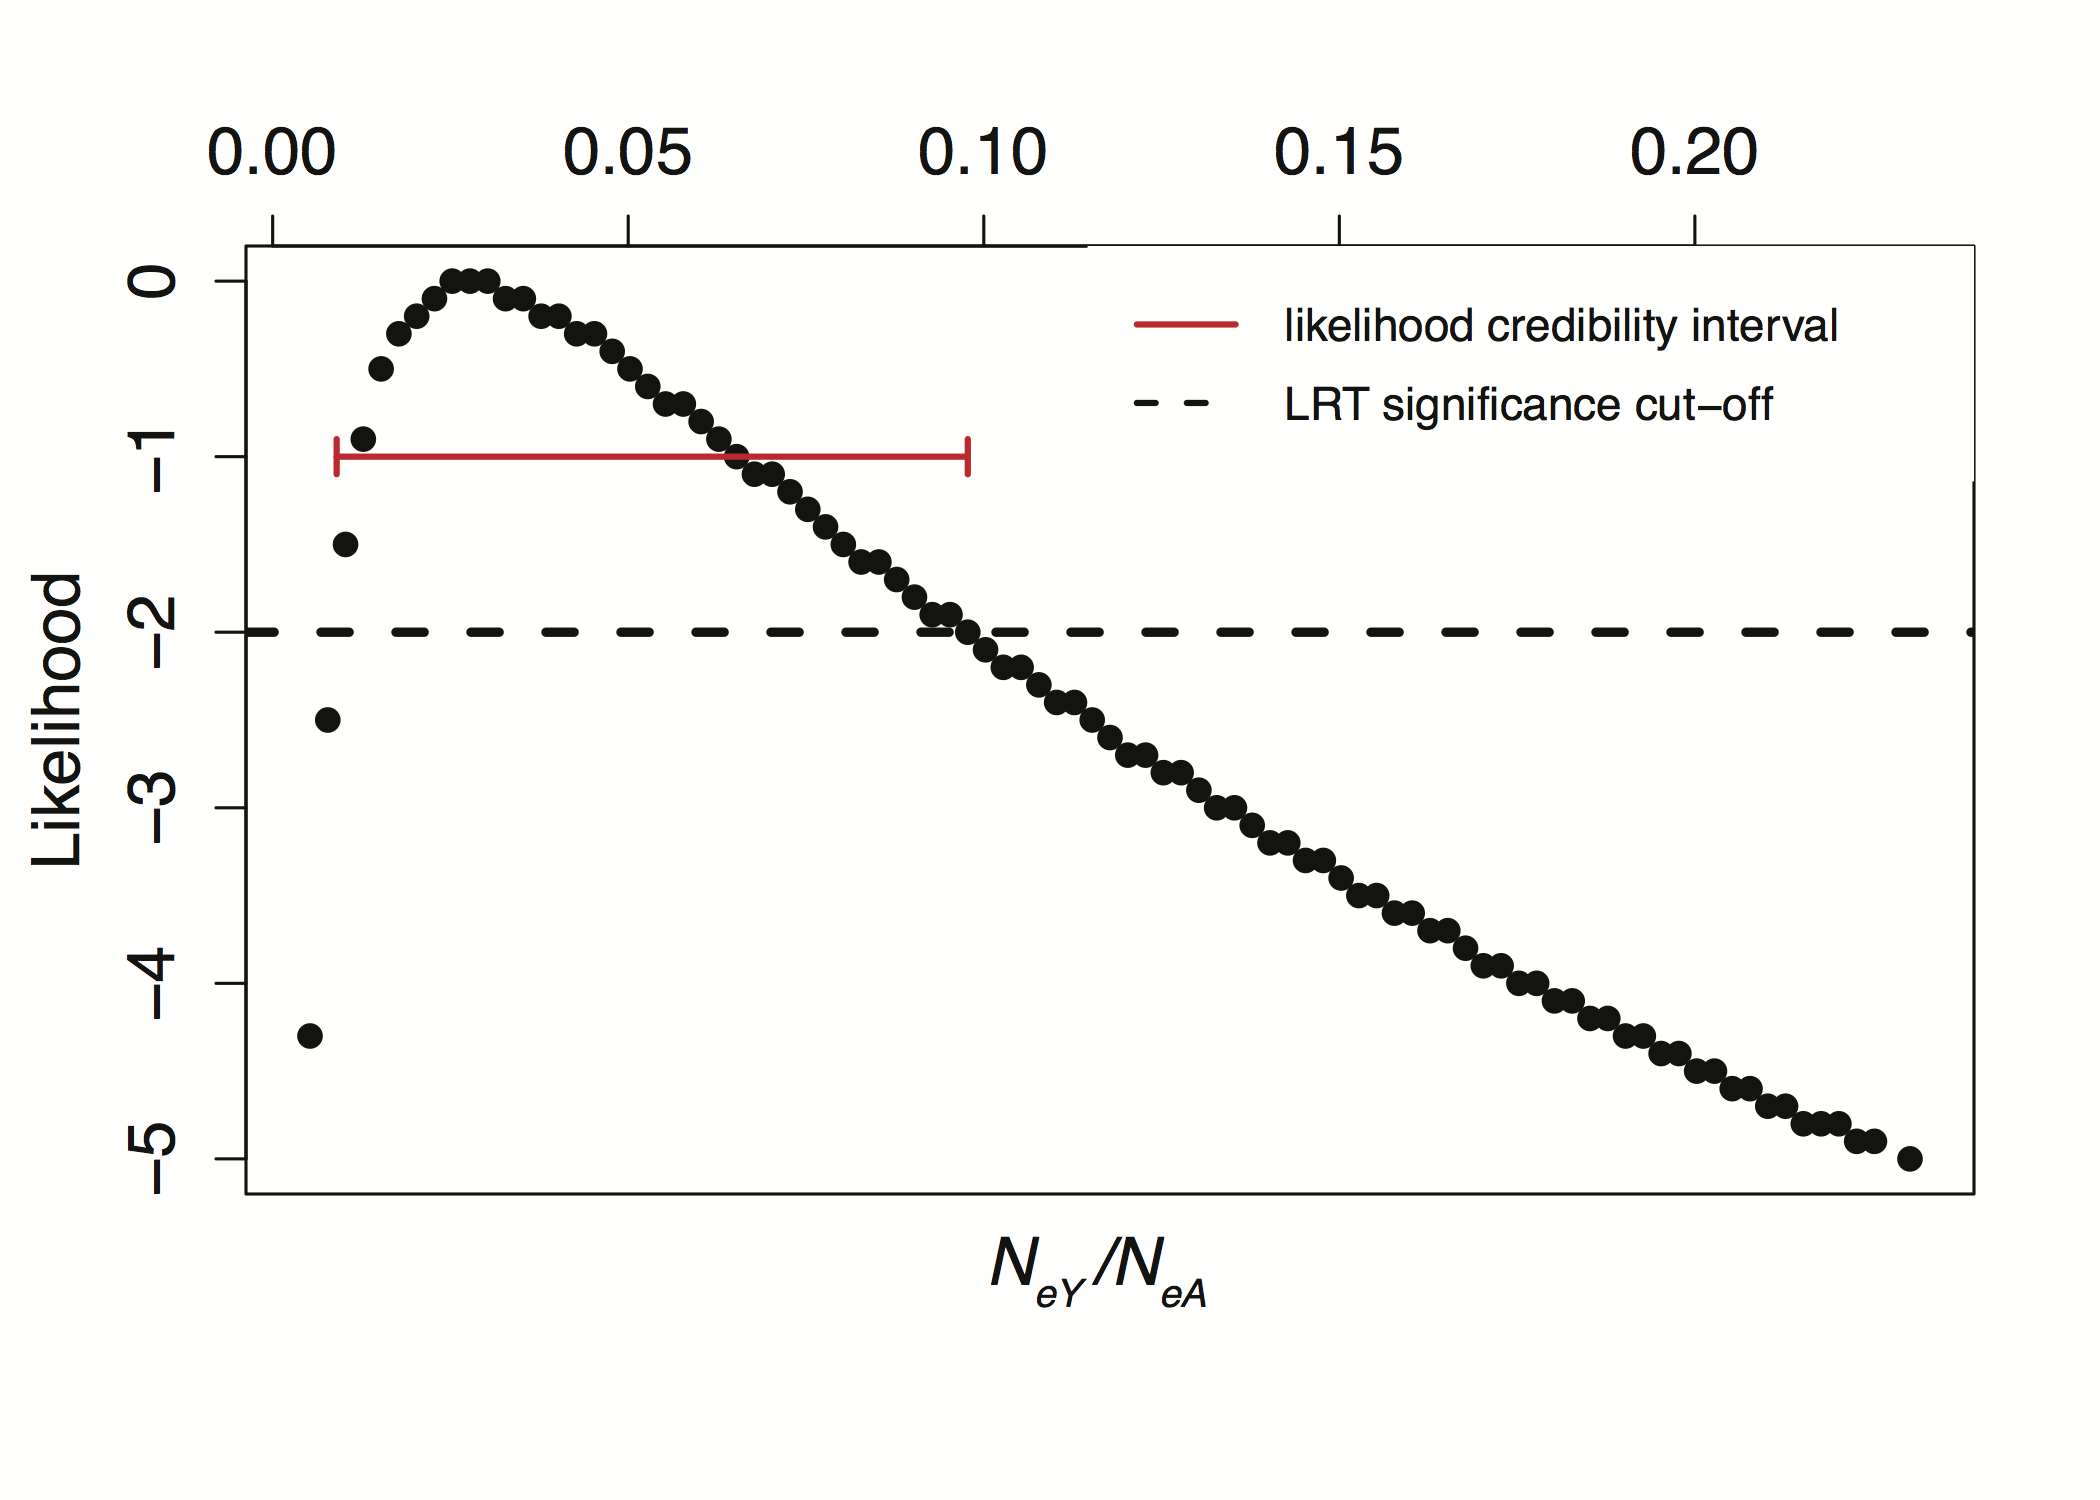
\includegraphics[width=.5\linewidth]{FigureS1.png}
\caption{likelihood estimation of the Y/A ratio}
\label{figure:FigureS1}
\end{figure}

\end{document}